% introduction chapitre 2
\subsubsection*{Remarque}
Dans ce chapitre, l'int�r�t sera pratiquement toujours \underline{compos�}.

\subsubsection*{Quelques d�finitions...}
\begin{description}
	\item[Rentes (\emph{annuities})]{s�rie de versements p�riodiques.}
	\item[Rente contingente]{conditionnel � la survie ou que l'entreprise 		reste ouverte.}
	\item[Rente certaine]{C'est s�r � 100\% qu'on recevra les versements 	(\emph{�a sera toujours le cas dans le cours ACT-1001})}
\end{description}	

\subsubsection{\hl{Rappel super important}}
La propri�t�s des sommes g�om�triques, \underline{TR�S IMPORTANT} pour les annuit�s!
\begin{empheq} [box=\fcolorbox{black}{green}]{equation}
\sum_{j=m}^n ar^j = ar^m \left(\frac{1-r^{n-m+1}}{1-r} \right)
\end{empheq}

\subsubsection{Exemple 2.1}
On re�oit des versements p�riodiques de 30\$/mois et on est capable d'obtenir un taux d'int�r�t nominal annuel compos� mensuellement ($i^{(12)}$) de 9\%. Quelle est la valeur accumul�e au moment du 140\up{e} versement?
% ------
\p
Tout d'abord, il est important de se faire un graphique : 
\begin{center}   % INSERTION D'UNE IMAGE POUR AIDER � comprendre
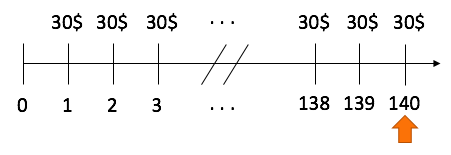
\includegraphics[width = 10cm, height = 4cm]{illustrations/ex2_1_chap2.png}
\end{center}
% ------
Ensuite, on convertit notre taux d'int�r�t pour le mettre sur la m�me fr�quence que nos versements : 

\begin{gather*}
\frac{i^{(12)}}{12} = \frac{0,09}{12} = 0,75\% \text{ par mois}
\end{gather*}

Apr�s, on doit trouver la valeur accumul�e de cette annuit� (s�rie de versements). Il s'ag�t d'une suite de versements qui peut �tre g�n�ralis�e comme suit : 

\begin{gather*}
30(1+0,0075)^{139} + 30(1+0,0075)^{138} + ... + 30(1+0,0075)^{2} + 30(1+0,0075)^{1} + 30
\end{gather*}

Avec la propri�t� des sommes g�om�triques, on est capable de r�soudre rapidement cette suite : 

\begin{gather*}
\sum_{m=1}^{139} 30(1+0,0075)^m = 30 \left(\frac{1- (1+0,0075)^{140}}{1-(1+0,0075)} \right) = 7385,91\$
\end{gather*}

